%----------------------------------------------------------
\chapter{Сборка и тестирование}
\label{ch:chap4_soft_testing}
%----------------------------------------------------------

В экосистеме языка Rust принято использовать Cargo~\cite{CargoBook} для сборки приложения, управления зависимостями и тестирования.
Для сборки прототипа компилятора Kodept тоже необходимо использовать этот инструмент.
На данный момент используется превью-версия 1.80.0 компилятора Rust для доступа к нестабильным функциям языка, что тоже необходимо учитывать при сборке.
Собрать проект можно выполнив следующую команду в командной строке:

\begin{verbatim}
    cargo build --release
\end{verbatim}

Пакетный менеджер Cargo скачает необходимые зависимости и соберёт программу.
Приложение выполняется кросс-платформенно, его работа была протестирована на ОС Linux и на ОС Windows.
Дополнительных требований к получаемому исполняемому файлу не предоставляется.

При разработке приложения не обойтись без тестирования.
Оно помогает выявить различные ошибки и исправить их.
Популярным вариантом тестирования является модульное тестирование (англ. unit тестирование).
Unit тест~--- функция или набор функций, которые проверяют корректность работы отдельной нетривиальной части программы.

В ходе разработки компилятора были написаны модульные тесты, они покрывают большое количество кода и успешно выполняются.
Для их запуска требуется Cargo с использованием следующей команды:

\begin{verbatim}
    cargo test --all --all-features --no-fail-fast
\end{verbatim}

Компилятор Kodept можно собрать с поддержкой профилирования использованной оперативной памяти.
Для этого можно воспользоваться отдельным механизмом Cargo~--- особенность (англ. feature).
Профилирование памяти помогает узнать использование оперативной памяти в разные моменты программы.
Так, например, для исходного кода с листинга~\ref{lst:kodept}, на рисунке~\ref{fig:profiling} показаны результаты профилирования используемой памяти компилятора.
Первые три строки вывода занимают логи о прохождении этапов компиляции.
Затем приведена информация о профилировании: за всё время работы было использовано 320Кб, максимальный размер~--- 61Кб, в момент завершения выполнения~--- 34Кб.

\begin{figure}[h]
    \centering
    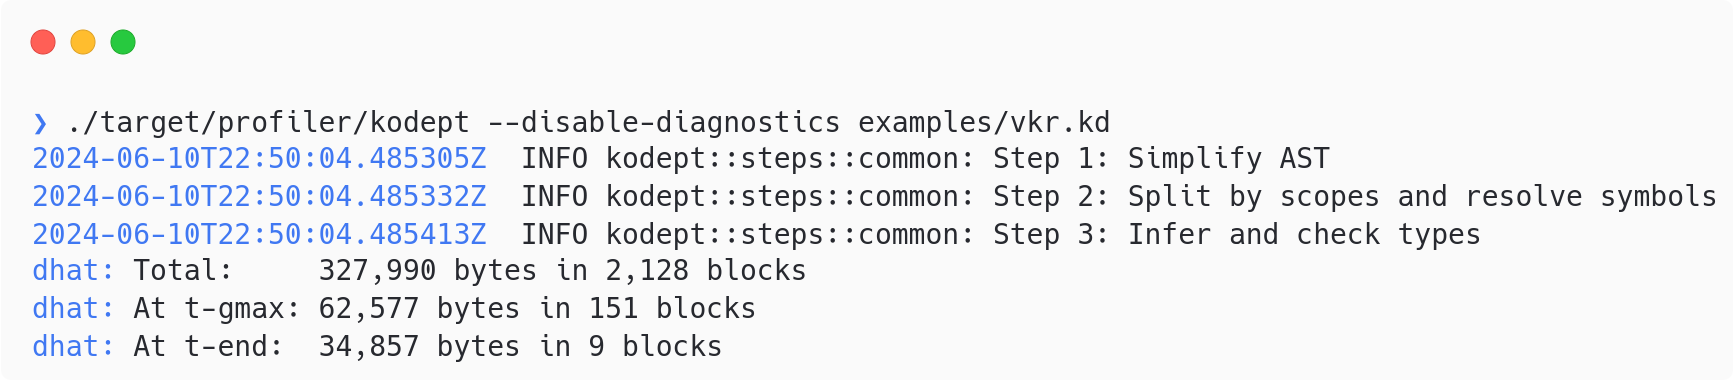
\includegraphics[width=\textwidth]{figures/profiling}
    \caption{Скриншот вывода компилятора Kodept при запуске с опцией профилирования}
    \label{fig:profiling}
\end{figure}

Рассмотрим теперь непосредственно работу вывода типов в программе.
Для исходного кода с листинга~\ref{lst:kodept} в разделе~\ref{subsec:ast_transformation} было сказано, что образованный из функции \lstinline{compose} терм $e$ выглядит так: $\lambda f. \lambda g. \lambda x. f(g(x))$.
Если воспользоваться алгоритмом $\mathcal{W}_c$, приведёнными в разделе~\ref{sec:inference_algo}, то тип $\tau$ терма $e$ будет следующим: $\forall \left\{ \alpha_1, \alpha_2, \alpha_3 \right\}. (\alpha_2 \to \alpha_3) \to (\alpha_1 \to \alpha_2) \to (\alpha_1 \to \alpha_3)$.
Действительно, тип этой функции, определённый компилятором совпадает с $\tau$ с точностью до имен переменных типа~\figref{fig:inferring}.

\begin{figure}
    \centering
    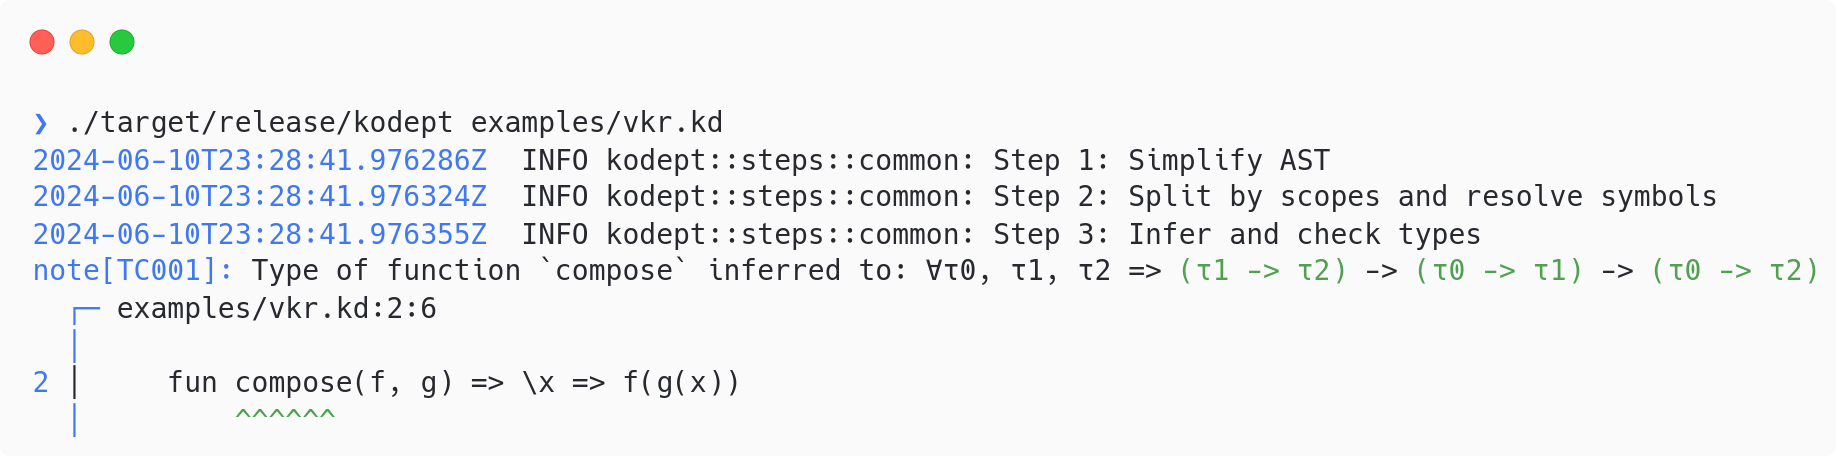
\includegraphics[width=\textwidth]{figures/inferring}
    \caption{Скриншот вывода компилятора Kodept с типом функции compose}
    \label{fig:inferring}
\end{figure}

%----------------------------------------------------------

